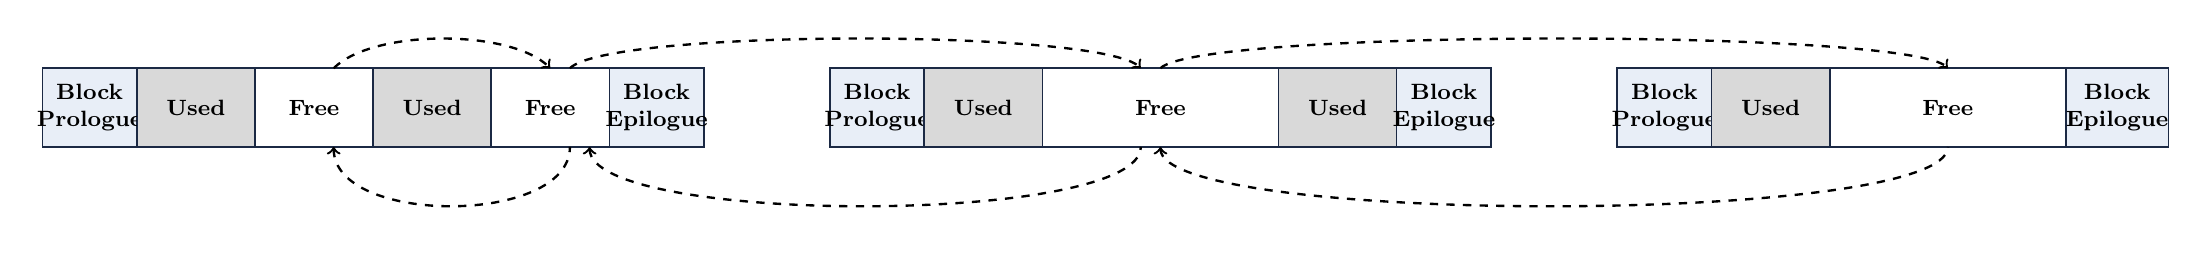
\begin{tikzpicture}

\definecolor{customColor1}{HTML}{B3C5E3}
\definecolor{customColor2}{HTML}{1B2944}
\definecolor{customColor3}{HTML}{7A944A}
\definecolor{customColor4}{HTML}{3D4A25}
\definecolor{customColor5}{RGB}{252,251,244}
% First diagram (initial state)
% Block Prologue (increased width)
\fill[customColor1!30, draw=customColor2!100, line width=0.2mm] (0, 0) rectangle (1.2, 1) coordinate (block1);
\node at (0.6, 0.5) [align=center, text=black, font=\footnotesize] {\textbf{Block}\\\textbf{Prologue}};

% Used
\fill[gray!30, draw=customColor2!100, line width=0.2mm] (1.21, 0) rectangle (2.7, 1) coordinate (used1);
\node at (1.95, 0.5) [text=black, font=\footnotesize] {\textbf{Used}};

% Free
\draw[fill=white, draw=customColor2!100, line width=0.2mm] (2.7, 0) rectangle (4.2, 1) coordinate (free1);
\node at (3.45, 0.5) [text=black, font=\footnotesize] {\textbf{Free}};

% Used
\fill[gray!30, draw=customColor2!100, line width=0.2mm] (4.2, 0) rectangle (5.7, 1) coordinate (used2);
\node at (4.95, 0.5) [text=black, font=\footnotesize] {\textbf{Used}};

% Free
\draw[fill=white, draw=customColor2!100, line width=0.2mm] (5.7, 0) rectangle (7.2, 1) coordinate (free2);
\node at (6.45, 0.5) [text=black, font=\footnotesize] {\textbf{Free}};

% Block Epilogue (increased width)
\fill[customColor1!30, draw=customColor2!100, line width=0.2mm] (7.2, 0) rectangle (8.4, 1) coordinate (block2);
\node at (7.8, 0.5) [align=center, text=black, font=\footnotesize] {\textbf{Block}\\\textbf{Epilogue}};

% Increase arrow size
% Arrow from free1 to free2 (shifted towards the middle)
\draw[->, thick, dashed, black, line width=0.3mm] ([xshift=-0.5cm]free1.east) .. controls +(0.5, 0.5) and +(-0.5, 0.5) .. ([xshift=-0.75cm]free2.west);

% Reverse arrow from free2 to free1 (from the bottom)
\draw[<-, thick, dashed, black, line width=0.3mm] ([xshift=-0.5cm, yshift=-1cm]free1.south) .. controls +(0, -1) and +(0, -1) .. ([xshift=-0.5cm, yshift=-1cm]free2.south);

% Second diagram (after merge of two free blocks)
% Block Prologue (increased width)
\fill[customColor1!30, draw=customColor2!100, line width=0.2mm] (10, 0) rectangle (11.2, 1) coordinate (block3);
\node at (10.6, 0.5) [align=center, text=black, font=\footnotesize] {\textbf{Block}\\\textbf{Prologue}};

% Used
\fill[gray!30, draw=customColor2!100, line width=0.2mm] (11.2, 0) rectangle (12.7, 1) coordinate (used3);
\node at (11.95, 0.5) [text=black, font=\footnotesize] {\textbf{Used}};

% Free (merged)
\draw[fill=white, draw=customColor2!100, line width=0.2mm] (12.7, 0) rectangle (15.7, 1) coordinate (free3);
\node at (14.2, 0.5) [text=black, font=\footnotesize] {\textbf{Free}};

% Used
\fill[gray!30, draw=customColor2!100, line width=0.2mm] (15.7, 0) rectangle (17.2, 1) coordinate (used4);
\node at (16.45, 0.5) [text=black, font=\footnotesize] {\textbf{Used}};

% Block Epilogue (increased width)
\fill[customColor1!30, draw=customColor2!100, line width=0.2mm] (17.2, 0) rectangle (18.4, 1) coordinate (block4);
\node at (17.8, 0.5) [align=center, text=black, font=\footnotesize] {\textbf{Block}\\\textbf{Epilogue}};

% Arrow from free2 to free3 (shifted towards the middle)
\draw[->, thick, dashed, line width=0.3mm] ([xshift=-0.5cm]free2.east) .. controls +(0.5, 0.5) and +(-0.5, 0.5) .. ([xshift=-1.75cm]free3.west);

% Reverse arrow from free3 to free2 (from the bottom)
\draw[<-, thick, dashed, black, line width=0.3mm] ([xshift=-0.25cm, yshift=-1cm]free2.south) .. controls +(0, -1) and +(0, -1) .. ([xshift=-1.75cm, yshift=-1cm]free3.south);

% Third diagram (after merging all free blocks)
% Block Prologue (increased width)
\fill[customColor1!30, draw=customColor2!100, line width=0.2mm] (20, 0) rectangle (21.2, 1) coordinate (block5);
\node at (20.6, 0.5) [align=center, text=black, font=\footnotesize] {\textbf{Block}\\\textbf{Prologue}};

% Used
\fill[gray!30, draw=customColor2!100, line width=0.2mm] (21.2, 0) rectangle (22.7, 1) coordinate (used5);
\node at (21.95, 0.5) [text=black, font=\footnotesize] {\textbf{Used}};

% Free (merged)
\draw[fill=white, draw=customColor2!100, line width=0.2mm] (22.7, 0) rectangle (25.7, 1) coordinate (free4);
\node at (24.2, 0.5) [text=black, font=\footnotesize] {\textbf{Free}};

% Block Epilogue (increased width)
\fill[customColor1!30, draw=customColor2!100, line width=0.2mm] (25.7, 0) rectangle (27, 1) coordinate (block6);
\node at (26.35, 0.5) [align=center, text=black, font=\footnotesize] {\textbf{Block}\\\textbf{Epilogue}};

% Arrow from free3 to free4 (shifted towards the middle)
\draw[->, thick, dashed, black, line width=0.3mm] ([xshift=-1.5cm]free3.east) .. controls +(0.5, 0.5) and +(-0.5, 0.5) .. ([xshift=-1.5cm]free4.west);

% Reverse arrow from free4 to free3 (from the bottom)
\draw[<-, thick, dashed, black, line width=0.3mm] ([xshift=-1.5cm, yshift=-1cm]free3.south) .. controls +(0, -1) and +(0, -1) .. ([xshift=-1.5cm, yshift=-1cm]free4.south);

\end{tikzpicture}
